
% Default to the notebook output style

    


% Inherit from the specified cell style.




    
\documentclass[11pt]{article}

    
    
    \usepackage[T1]{fontenc}
    % Nicer default font (+ math font) than Computer Modern for most use cases
    \usepackage{mathpazo}

    % Basic figure setup, for now with no caption control since it's done
    % automatically by Pandoc (which extracts ![](path) syntax from Markdown).
    \usepackage{graphicx}
    % We will generate all images so they have a width \maxwidth. This means
    % that they will get their normal width if they fit onto the page, but
    % are scaled down if they would overflow the margins.
    \makeatletter
    \def\maxwidth{\ifdim\Gin@nat@width>\linewidth\linewidth
    \else\Gin@nat@width\fi}
    \makeatother
    \let\Oldincludegraphics\includegraphics
    % Set max figure width to be 80% of text width, for now hardcoded.
    \renewcommand{\includegraphics}[1]{\Oldincludegraphics[width=.8\maxwidth]{#1}}
    % Ensure that by default, figures have no caption (until we provide a
    % proper Figure object with a Caption API and a way to capture that
    % in the conversion process - todo).
    \usepackage{caption}
    \DeclareCaptionLabelFormat{nolabel}{}
    \captionsetup{labelformat=nolabel}

    \usepackage{adjustbox} % Used to constrain images to a maximum size 
    \usepackage{xcolor} % Allow colors to be defined
    \usepackage{enumerate} % Needed for markdown enumerations to work
    \usepackage{geometry} % Used to adjust the document margins
    \usepackage{amsmath} % Equations
    \usepackage{amssymb} % Equations
    \usepackage{textcomp} % defines textquotesingle
    % Hack from http://tex.stackexchange.com/a/47451/13684:
    \AtBeginDocument{%
        \def\PYZsq{\textquotesingle}% Upright quotes in Pygmentized code
    }
    \usepackage{upquote} % Upright quotes for verbatim code
    \usepackage{eurosym} % defines \euro
    \usepackage[mathletters]{ucs} % Extended unicode (utf-8) support
    \usepackage[utf8x]{inputenc} % Allow utf-8 characters in the tex document
    \usepackage{fancyvrb} % verbatim replacement that allows latex
    \usepackage{grffile} % extends the file name processing of package graphics 
                         % to support a larger range 
    % The hyperref package gives us a pdf with properly built
    % internal navigation ('pdf bookmarks' for the table of contents,
    % internal cross-reference links, web links for URLs, etc.)
    \usepackage{hyperref}
    \usepackage{longtable} % longtable support required by pandoc >1.10
    \usepackage{booktabs}  % table support for pandoc > 1.12.2
    \usepackage[inline]{enumitem} % IRkernel/repr support (it uses the enumerate* environment)
    \usepackage[normalem]{ulem} % ulem is needed to support strikethroughs (\sout)
                                % normalem makes italics be italics, not underlines
    

    
    
    % Colors for the hyperref package
    \definecolor{urlcolor}{rgb}{0,.145,.698}
    \definecolor{linkcolor}{rgb}{.71,0.21,0.01}
    \definecolor{citecolor}{rgb}{.12,.54,.11}

    % ANSI colors
    \definecolor{ansi-black}{HTML}{3E424D}
    \definecolor{ansi-black-intense}{HTML}{282C36}
    \definecolor{ansi-red}{HTML}{E75C58}
    \definecolor{ansi-red-intense}{HTML}{B22B31}
    \definecolor{ansi-green}{HTML}{00A250}
    \definecolor{ansi-green-intense}{HTML}{007427}
    \definecolor{ansi-yellow}{HTML}{DDB62B}
    \definecolor{ansi-yellow-intense}{HTML}{B27D12}
    \definecolor{ansi-blue}{HTML}{208FFB}
    \definecolor{ansi-blue-intense}{HTML}{0065CA}
    \definecolor{ansi-magenta}{HTML}{D160C4}
    \definecolor{ansi-magenta-intense}{HTML}{A03196}
    \definecolor{ansi-cyan}{HTML}{60C6C8}
    \definecolor{ansi-cyan-intense}{HTML}{258F8F}
    \definecolor{ansi-white}{HTML}{C5C1B4}
    \definecolor{ansi-white-intense}{HTML}{A1A6B2}

    % commands and environments needed by pandoc snippets
    % extracted from the output of `pandoc -s`
    \providecommand{\tightlist}{%
      \setlength{\itemsep}{0pt}\setlength{\parskip}{0pt}}
    \DefineVerbatimEnvironment{Highlighting}{Verbatim}{commandchars=\\\{\}}
    % Add ',fontsize=\small' for more characters per line
    \newenvironment{Shaded}{}{}
    \newcommand{\KeywordTok}[1]{\textcolor[rgb]{0.00,0.44,0.13}{\textbf{{#1}}}}
    \newcommand{\DataTypeTok}[1]{\textcolor[rgb]{0.56,0.13,0.00}{{#1}}}
    \newcommand{\DecValTok}[1]{\textcolor[rgb]{0.25,0.63,0.44}{{#1}}}
    \newcommand{\BaseNTok}[1]{\textcolor[rgb]{0.25,0.63,0.44}{{#1}}}
    \newcommand{\FloatTok}[1]{\textcolor[rgb]{0.25,0.63,0.44}{{#1}}}
    \newcommand{\CharTok}[1]{\textcolor[rgb]{0.25,0.44,0.63}{{#1}}}
    \newcommand{\StringTok}[1]{\textcolor[rgb]{0.25,0.44,0.63}{{#1}}}
    \newcommand{\CommentTok}[1]{\textcolor[rgb]{0.38,0.63,0.69}{\textit{{#1}}}}
    \newcommand{\OtherTok}[1]{\textcolor[rgb]{0.00,0.44,0.13}{{#1}}}
    \newcommand{\AlertTok}[1]{\textcolor[rgb]{1.00,0.00,0.00}{\textbf{{#1}}}}
    \newcommand{\FunctionTok}[1]{\textcolor[rgb]{0.02,0.16,0.49}{{#1}}}
    \newcommand{\RegionMarkerTok}[1]{{#1}}
    \newcommand{\ErrorTok}[1]{\textcolor[rgb]{1.00,0.00,0.00}{\textbf{{#1}}}}
    \newcommand{\NormalTok}[1]{{#1}}
    
    % Additional commands for more recent versions of Pandoc
    \newcommand{\ConstantTok}[1]{\textcolor[rgb]{0.53,0.00,0.00}{{#1}}}
    \newcommand{\SpecialCharTok}[1]{\textcolor[rgb]{0.25,0.44,0.63}{{#1}}}
    \newcommand{\VerbatimStringTok}[1]{\textcolor[rgb]{0.25,0.44,0.63}{{#1}}}
    \newcommand{\SpecialStringTok}[1]{\textcolor[rgb]{0.73,0.40,0.53}{{#1}}}
    \newcommand{\ImportTok}[1]{{#1}}
    \newcommand{\DocumentationTok}[1]{\textcolor[rgb]{0.73,0.13,0.13}{\textit{{#1}}}}
    \newcommand{\AnnotationTok}[1]{\textcolor[rgb]{0.38,0.63,0.69}{\textbf{\textit{{#1}}}}}
    \newcommand{\CommentVarTok}[1]{\textcolor[rgb]{0.38,0.63,0.69}{\textbf{\textit{{#1}}}}}
    \newcommand{\VariableTok}[1]{\textcolor[rgb]{0.10,0.09,0.49}{{#1}}}
    \newcommand{\ControlFlowTok}[1]{\textcolor[rgb]{0.00,0.44,0.13}{\textbf{{#1}}}}
    \newcommand{\OperatorTok}[1]{\textcolor[rgb]{0.40,0.40,0.40}{{#1}}}
    \newcommand{\BuiltInTok}[1]{{#1}}
    \newcommand{\ExtensionTok}[1]{{#1}}
    \newcommand{\PreprocessorTok}[1]{\textcolor[rgb]{0.74,0.48,0.00}{{#1}}}
    \newcommand{\AttributeTok}[1]{\textcolor[rgb]{0.49,0.56,0.16}{{#1}}}
    \newcommand{\InformationTok}[1]{\textcolor[rgb]{0.38,0.63,0.69}{\textbf{\textit{{#1}}}}}
    \newcommand{\WarningTok}[1]{\textcolor[rgb]{0.38,0.63,0.69}{\textbf{\textit{{#1}}}}}
    
    
    % Define a nice break command that doesn't care if a line doesn't already
    % exist.
    \def\br{\hspace*{\fill} \\* }
    % Math Jax compatability definitions
    \def\gt{>}
    \def\lt{<}
    % Document parameters
    \title{sheet1 - solution group SSASCD}
    \author{Karel Smejkal\\
							Darya Smirnova\\
							Mohammad Abdelkhalek\\
							Michael Samuels\\
							Julián Cantor\\
							Marta Domagalska}
    
    
    

    % Pygments definitions
    
\makeatletter
\def\PY@reset{\let\PY@it=\relax \let\PY@bf=\relax%
    \let\PY@ul=\relax \let\PY@tc=\relax%
    \let\PY@bc=\relax \let\PY@ff=\relax}
\def\PY@tok#1{\csname PY@tok@#1\endcsname}
\def\PY@toks#1+{\ifx\relax#1\empty\else%
    \PY@tok{#1}\expandafter\PY@toks\fi}
\def\PY@do#1{\PY@bc{\PY@tc{\PY@ul{%
    \PY@it{\PY@bf{\PY@ff{#1}}}}}}}
\def\PY#1#2{\PY@reset\PY@toks#1+\relax+\PY@do{#2}}

\expandafter\def\csname PY@tok@w\endcsname{\def\PY@tc##1{\textcolor[rgb]{0.73,0.73,0.73}{##1}}}
\expandafter\def\csname PY@tok@c\endcsname{\let\PY@it=\textit\def\PY@tc##1{\textcolor[rgb]{0.25,0.50,0.50}{##1}}}
\expandafter\def\csname PY@tok@cp\endcsname{\def\PY@tc##1{\textcolor[rgb]{0.74,0.48,0.00}{##1}}}
\expandafter\def\csname PY@tok@k\endcsname{\let\PY@bf=\textbf\def\PY@tc##1{\textcolor[rgb]{0.00,0.50,0.00}{##1}}}
\expandafter\def\csname PY@tok@kp\endcsname{\def\PY@tc##1{\textcolor[rgb]{0.00,0.50,0.00}{##1}}}
\expandafter\def\csname PY@tok@kt\endcsname{\def\PY@tc##1{\textcolor[rgb]{0.69,0.00,0.25}{##1}}}
\expandafter\def\csname PY@tok@o\endcsname{\def\PY@tc##1{\textcolor[rgb]{0.40,0.40,0.40}{##1}}}
\expandafter\def\csname PY@tok@ow\endcsname{\let\PY@bf=\textbf\def\PY@tc##1{\textcolor[rgb]{0.67,0.13,1.00}{##1}}}
\expandafter\def\csname PY@tok@nb\endcsname{\def\PY@tc##1{\textcolor[rgb]{0.00,0.50,0.00}{##1}}}
\expandafter\def\csname PY@tok@nf\endcsname{\def\PY@tc##1{\textcolor[rgb]{0.00,0.00,1.00}{##1}}}
\expandafter\def\csname PY@tok@nc\endcsname{\let\PY@bf=\textbf\def\PY@tc##1{\textcolor[rgb]{0.00,0.00,1.00}{##1}}}
\expandafter\def\csname PY@tok@nn\endcsname{\let\PY@bf=\textbf\def\PY@tc##1{\textcolor[rgb]{0.00,0.00,1.00}{##1}}}
\expandafter\def\csname PY@tok@ne\endcsname{\let\PY@bf=\textbf\def\PY@tc##1{\textcolor[rgb]{0.82,0.25,0.23}{##1}}}
\expandafter\def\csname PY@tok@nv\endcsname{\def\PY@tc##1{\textcolor[rgb]{0.10,0.09,0.49}{##1}}}
\expandafter\def\csname PY@tok@no\endcsname{\def\PY@tc##1{\textcolor[rgb]{0.53,0.00,0.00}{##1}}}
\expandafter\def\csname PY@tok@nl\endcsname{\def\PY@tc##1{\textcolor[rgb]{0.63,0.63,0.00}{##1}}}
\expandafter\def\csname PY@tok@ni\endcsname{\let\PY@bf=\textbf\def\PY@tc##1{\textcolor[rgb]{0.60,0.60,0.60}{##1}}}
\expandafter\def\csname PY@tok@na\endcsname{\def\PY@tc##1{\textcolor[rgb]{0.49,0.56,0.16}{##1}}}
\expandafter\def\csname PY@tok@nt\endcsname{\let\PY@bf=\textbf\def\PY@tc##1{\textcolor[rgb]{0.00,0.50,0.00}{##1}}}
\expandafter\def\csname PY@tok@nd\endcsname{\def\PY@tc##1{\textcolor[rgb]{0.67,0.13,1.00}{##1}}}
\expandafter\def\csname PY@tok@s\endcsname{\def\PY@tc##1{\textcolor[rgb]{0.73,0.13,0.13}{##1}}}
\expandafter\def\csname PY@tok@sd\endcsname{\let\PY@it=\textit\def\PY@tc##1{\textcolor[rgb]{0.73,0.13,0.13}{##1}}}
\expandafter\def\csname PY@tok@si\endcsname{\let\PY@bf=\textbf\def\PY@tc##1{\textcolor[rgb]{0.73,0.40,0.53}{##1}}}
\expandafter\def\csname PY@tok@se\endcsname{\let\PY@bf=\textbf\def\PY@tc##1{\textcolor[rgb]{0.73,0.40,0.13}{##1}}}
\expandafter\def\csname PY@tok@sr\endcsname{\def\PY@tc##1{\textcolor[rgb]{0.73,0.40,0.53}{##1}}}
\expandafter\def\csname PY@tok@ss\endcsname{\def\PY@tc##1{\textcolor[rgb]{0.10,0.09,0.49}{##1}}}
\expandafter\def\csname PY@tok@sx\endcsname{\def\PY@tc##1{\textcolor[rgb]{0.00,0.50,0.00}{##1}}}
\expandafter\def\csname PY@tok@m\endcsname{\def\PY@tc##1{\textcolor[rgb]{0.40,0.40,0.40}{##1}}}
\expandafter\def\csname PY@tok@gh\endcsname{\let\PY@bf=\textbf\def\PY@tc##1{\textcolor[rgb]{0.00,0.00,0.50}{##1}}}
\expandafter\def\csname PY@tok@gu\endcsname{\let\PY@bf=\textbf\def\PY@tc##1{\textcolor[rgb]{0.50,0.00,0.50}{##1}}}
\expandafter\def\csname PY@tok@gd\endcsname{\def\PY@tc##1{\textcolor[rgb]{0.63,0.00,0.00}{##1}}}
\expandafter\def\csname PY@tok@gi\endcsname{\def\PY@tc##1{\textcolor[rgb]{0.00,0.63,0.00}{##1}}}
\expandafter\def\csname PY@tok@gr\endcsname{\def\PY@tc##1{\textcolor[rgb]{1.00,0.00,0.00}{##1}}}
\expandafter\def\csname PY@tok@ge\endcsname{\let\PY@it=\textit}
\expandafter\def\csname PY@tok@gs\endcsname{\let\PY@bf=\textbf}
\expandafter\def\csname PY@tok@gp\endcsname{\let\PY@bf=\textbf\def\PY@tc##1{\textcolor[rgb]{0.00,0.00,0.50}{##1}}}
\expandafter\def\csname PY@tok@go\endcsname{\def\PY@tc##1{\textcolor[rgb]{0.53,0.53,0.53}{##1}}}
\expandafter\def\csname PY@tok@gt\endcsname{\def\PY@tc##1{\textcolor[rgb]{0.00,0.27,0.87}{##1}}}
\expandafter\def\csname PY@tok@err\endcsname{\def\PY@bc##1{\setlength{\fboxsep}{0pt}\fcolorbox[rgb]{1.00,0.00,0.00}{1,1,1}{\strut ##1}}}
\expandafter\def\csname PY@tok@kc\endcsname{\let\PY@bf=\textbf\def\PY@tc##1{\textcolor[rgb]{0.00,0.50,0.00}{##1}}}
\expandafter\def\csname PY@tok@kd\endcsname{\let\PY@bf=\textbf\def\PY@tc##1{\textcolor[rgb]{0.00,0.50,0.00}{##1}}}
\expandafter\def\csname PY@tok@kn\endcsname{\let\PY@bf=\textbf\def\PY@tc##1{\textcolor[rgb]{0.00,0.50,0.00}{##1}}}
\expandafter\def\csname PY@tok@kr\endcsname{\let\PY@bf=\textbf\def\PY@tc##1{\textcolor[rgb]{0.00,0.50,0.00}{##1}}}
\expandafter\def\csname PY@tok@bp\endcsname{\def\PY@tc##1{\textcolor[rgb]{0.00,0.50,0.00}{##1}}}
\expandafter\def\csname PY@tok@fm\endcsname{\def\PY@tc##1{\textcolor[rgb]{0.00,0.00,1.00}{##1}}}
\expandafter\def\csname PY@tok@vc\endcsname{\def\PY@tc##1{\textcolor[rgb]{0.10,0.09,0.49}{##1}}}
\expandafter\def\csname PY@tok@vg\endcsname{\def\PY@tc##1{\textcolor[rgb]{0.10,0.09,0.49}{##1}}}
\expandafter\def\csname PY@tok@vi\endcsname{\def\PY@tc##1{\textcolor[rgb]{0.10,0.09,0.49}{##1}}}
\expandafter\def\csname PY@tok@vm\endcsname{\def\PY@tc##1{\textcolor[rgb]{0.10,0.09,0.49}{##1}}}
\expandafter\def\csname PY@tok@sa\endcsname{\def\PY@tc##1{\textcolor[rgb]{0.73,0.13,0.13}{##1}}}
\expandafter\def\csname PY@tok@sb\endcsname{\def\PY@tc##1{\textcolor[rgb]{0.73,0.13,0.13}{##1}}}
\expandafter\def\csname PY@tok@sc\endcsname{\def\PY@tc##1{\textcolor[rgb]{0.73,0.13,0.13}{##1}}}
\expandafter\def\csname PY@tok@dl\endcsname{\def\PY@tc##1{\textcolor[rgb]{0.73,0.13,0.13}{##1}}}
\expandafter\def\csname PY@tok@s2\endcsname{\def\PY@tc##1{\textcolor[rgb]{0.73,0.13,0.13}{##1}}}
\expandafter\def\csname PY@tok@sh\endcsname{\def\PY@tc##1{\textcolor[rgb]{0.73,0.13,0.13}{##1}}}
\expandafter\def\csname PY@tok@s1\endcsname{\def\PY@tc##1{\textcolor[rgb]{0.73,0.13,0.13}{##1}}}
\expandafter\def\csname PY@tok@mb\endcsname{\def\PY@tc##1{\textcolor[rgb]{0.40,0.40,0.40}{##1}}}
\expandafter\def\csname PY@tok@mf\endcsname{\def\PY@tc##1{\textcolor[rgb]{0.40,0.40,0.40}{##1}}}
\expandafter\def\csname PY@tok@mh\endcsname{\def\PY@tc##1{\textcolor[rgb]{0.40,0.40,0.40}{##1}}}
\expandafter\def\csname PY@tok@mi\endcsname{\def\PY@tc##1{\textcolor[rgb]{0.40,0.40,0.40}{##1}}}
\expandafter\def\csname PY@tok@il\endcsname{\def\PY@tc##1{\textcolor[rgb]{0.40,0.40,0.40}{##1}}}
\expandafter\def\csname PY@tok@mo\endcsname{\def\PY@tc##1{\textcolor[rgb]{0.40,0.40,0.40}{##1}}}
\expandafter\def\csname PY@tok@ch\endcsname{\let\PY@it=\textit\def\PY@tc##1{\textcolor[rgb]{0.25,0.50,0.50}{##1}}}
\expandafter\def\csname PY@tok@cm\endcsname{\let\PY@it=\textit\def\PY@tc##1{\textcolor[rgb]{0.25,0.50,0.50}{##1}}}
\expandafter\def\csname PY@tok@cpf\endcsname{\let\PY@it=\textit\def\PY@tc##1{\textcolor[rgb]{0.25,0.50,0.50}{##1}}}
\expandafter\def\csname PY@tok@c1\endcsname{\let\PY@it=\textit\def\PY@tc##1{\textcolor[rgb]{0.25,0.50,0.50}{##1}}}
\expandafter\def\csname PY@tok@cs\endcsname{\let\PY@it=\textit\def\PY@tc##1{\textcolor[rgb]{0.25,0.50,0.50}{##1}}}

\def\PYZbs{\char`\\}
\def\PYZus{\char`\_}
\def\PYZob{\char`\{}
\def\PYZcb{\char`\}}
\def\PYZca{\char`\^}
\def\PYZam{\char`\&}
\def\PYZlt{\char`\<}
\def\PYZgt{\char`\>}
\def\PYZsh{\char`\#}
\def\PYZpc{\char`\%}
\def\PYZdl{\char`\$}
\def\PYZhy{\char`\-}
\def\PYZsq{\char`\'}
\def\PYZdq{\char`\"}
\def\PYZti{\char`\~}
% for compatibility with earlier versions
\def\PYZat{@}
\def\PYZlb{[}
\def\PYZrb{]}
\makeatother


    % Exact colors from NB
    \definecolor{incolor}{rgb}{0.0, 0.0, 0.5}
    \definecolor{outcolor}{rgb}{0.545, 0.0, 0.0}



    
    % Prevent overflowing lines due to hard-to-break entities
    \sloppy 
    % Setup hyperref package
    \hypersetup{
      breaklinks=true,  % so long urls are correctly broken across lines
      colorlinks=true,
      urlcolor=urlcolor,
      linkcolor=linkcolor,
      citecolor=citecolor,
      }
    % Slightly bigger margins than the latex defaults
    
    \geometry{verbose,tmargin=1in,bmargin=1in,lmargin=1in,rmargin=1in}
    
    

    \begin{document}
    
    
    \maketitle
    
    

    
    \section{Exercise Sheet 1: Python
Basics}\label{exercise-sheet-1-python-basics}

This first exercise sheet tests the basic functionalities of the Python
programming language in the context of a simple prediction task. We
consider the problem of predicting health risk of subjects from personal
data and habits. We first use for this task a decision tree

\begin{figure}
\centering
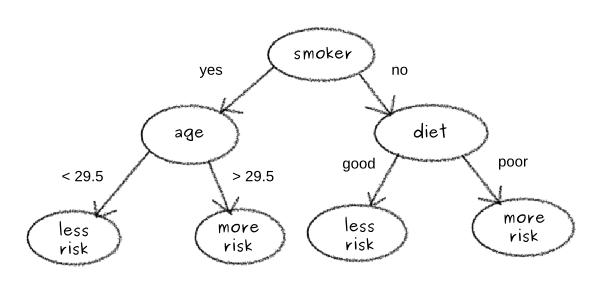
\includegraphics{tree.png}
\caption{}
\end{figure}

adapted from the webpage
http://www.refactorthis.net/post/2013/04/10/Machine-Learning-tutorial-How-to-create-a-decision-tree-in-RapidMiner-using-the-Titanic-passenger-data-set.aspx.
For this exercise sheet, you are required to use only pure Python, and
to not import any module, including numpy. In exercise sheet 2, the
nearest neighbor part of this exercise sheet will be revisited with
numpy.

    \subsection{Classifying a single instance (15
P)}\label{classifying-a-single-instance-15-p}

\begin{itemize}
\tightlist
\item
  Create a function that takes as input a tuple containing values for
  attributes (smoker,age,diet), and computes the output of the decision
  tree.
\item
  Test your function on the tuple
  \texttt{(\textquotesingle{}yes\textquotesingle{},31,\textquotesingle{}good\textquotesingle{})},
\end{itemize}

    \begin{Verbatim}[commandchars=\\\{\}]
{\color{incolor}In [{\color{incolor}1}]:} \PY{k}{def} \PY{n+nf}{exercise1}\PY{p}{(}\PY{n}{x}\PY{p}{)}\PY{p}{:}
                \PY{n}{result} \PY{o}{=} \PY{p}{[}\PY{p}{]}
                \PY{k}{if} \PY{n}{x}\PY{p}{[}\PY{l+m+mi}{0}\PY{p}{]} \PY{o}{==} \PY{l+s+s1}{\PYZsq{}}\PY{l+s+s1}{yes}\PY{l+s+s1}{\PYZsq{}}\PY{p}{:}
                    \PY{k}{if} \PY{n}{x}\PY{p}{[}\PY{l+m+mi}{1}\PY{p}{]} \PY{o}{\PYZgt{}} \PY{l+m+mf}{29.5}\PY{p}{:}
                        \PY{n}{decision} \PY{o}{=} \PY{l+s+s1}{\PYZsq{}}\PY{l+s+s1}{more}\PY{l+s+s1}{\PYZsq{}}
                    \PY{k}{else}\PY{p}{:}
                        \PY{n}{decision} \PY{o}{=} \PY{l+s+s1}{\PYZsq{}}\PY{l+s+s1}{less}\PY{l+s+s1}{\PYZsq{}}
                \PY{k}{else}\PY{p}{:}
                    \PY{k}{if} \PY{n}{x}\PY{p}{[}\PY{l+m+mi}{2}\PY{p}{]} \PY{o}{==} \PY{l+s+s1}{\PYZsq{}}\PY{l+s+s1}{poor}\PY{l+s+s1}{\PYZsq{}}\PY{p}{:}
                        \PY{n}{decision} \PY{o}{=} \PY{l+s+s1}{\PYZsq{}}\PY{l+s+s1}{more}\PY{l+s+s1}{\PYZsq{}}
                    \PY{k}{else}\PY{p}{:}
                        \PY{n}{decision} \PY{o}{=} \PY{l+s+s1}{\PYZsq{}}\PY{l+s+s1}{less}\PY{l+s+s1}{\PYZsq{}}
                \PY{n}{result}\PY{o}{.}\PY{n}{append}\PY{p}{(}\PY{p}{(}\PY{p}{(}\PY{n}{x}\PY{p}{[}\PY{l+m+mi}{0}\PY{p}{]}\PY{p}{,}\PY{n}{x}\PY{p}{[}\PY{l+m+mi}{1}\PY{p}{]}\PY{p}{,}\PY{n}{x}\PY{p}{[}\PY{l+m+mi}{2}\PY{p}{]}\PY{p}{)}\PY{p}{,}\PY{n}{decision}\PY{p}{)}\PY{p}{)}
                \PY{k}{return} \PY{n}{result}
        
        \PY{n}{exercise1}\PY{p}{(}\PY{p}{(}\PY{l+s+s1}{\PYZsq{}}\PY{l+s+s1}{yes}\PY{l+s+s1}{\PYZsq{}}\PY{p}{,}\PY{l+m+mi}{31}\PY{p}{,}\PY{l+s+s1}{\PYZsq{}}\PY{l+s+s1}{good}\PY{l+s+s1}{\PYZsq{}}\PY{p}{)}\PY{p}{)}
\end{Verbatim}


\begin{Verbatim}[commandchars=\\\{\}]
{\color{outcolor}Out[{\color{outcolor}1}]:} [(('yes', 31, 'good'), 'more')]
\end{Verbatim}
            
    \subsection{Reading a dataset from a text file (10
P)}\label{reading-a-dataset-from-a-text-file-10-p}

The file \texttt{health-test.txt} contains several fictious records of
personal data and habits.

\begin{itemize}
\tightlist
\item
  Read the file automatically using the methods introduced during the
  lecture.
\item
  Represent the dataset as a list of tuples.
\end{itemize}

    \begin{Verbatim}[commandchars=\\\{\}]
{\color{incolor}In [{\color{incolor}2}]:} \PY{k}{def} \PY{n+nf}{exercise2}\PY{p}{(}\PY{p}{)}\PY{p}{:}
            \PY{n}{f} \PY{o}{=} \PY{n+nb}{open}\PY{p}{(}\PY{l+s+s1}{\PYZsq{}}\PY{l+s+s1}{health\PYZhy{}test.txt}\PY{l+s+s1}{\PYZsq{}}\PY{p}{,}\PY{l+s+s1}{\PYZsq{}}\PY{l+s+s1}{r}\PY{l+s+s1}{\PYZsq{}}\PY{p}{)}
            \PY{n}{L} \PY{o}{=} \PY{p}{[}\PY{p}{]}
            \PY{k}{for} \PY{n}{line} \PY{o+ow}{in} \PY{n}{f}\PY{p}{:}
                \PY{n}{elem} \PY{o}{=} \PY{n}{line}\PY{p}{[}\PY{p}{:}\PY{o}{\PYZhy{}}\PY{l+m+mi}{1}\PY{p}{]}\PY{o}{.}\PY{n}{split}\PY{p}{(}\PY{l+s+s1}{\PYZsq{}}\PY{l+s+s1}{,}\PY{l+s+s1}{\PYZsq{}}\PY{p}{)}
                \PY{c+c1}{\PYZsh{}L += [(elem[0],float(elem[1]),elem[2])]}
                \PY{k}{if} \PY{n+nb}{float}\PY{p}{(}\PY{n}{elem}\PY{p}{[}\PY{l+m+mi}{1}\PY{p}{]}\PY{p}{)}\PY{o}{\PYZpc{}}\PY{k}{1} == 0:
                    \PY{n}{age} \PY{o}{=} \PY{n+nb}{int}\PY{p}{(}\PY{n}{elem}\PY{p}{[}\PY{l+m+mi}{1}\PY{p}{]}\PY{p}{)}
                \PY{k}{else}\PY{p}{:}
                    \PY{n}{age} \PY{o}{=} \PY{n+nb}{float}\PY{p}{(}\PY{n}{elem}\PY{p}{[}\PY{l+m+mi}{1}\PY{p}{]}\PY{p}{)}
                \PY{n}{L}\PY{o}{.}\PY{n}{append}\PY{p}{(}\PY{p}{(}\PY{n}{elem}\PY{p}{[}\PY{l+m+mi}{0}\PY{p}{]}\PY{p}{,}\PY{n}{age}\PY{p}{,}\PY{n}{elem}\PY{p}{[}\PY{l+m+mi}{2}\PY{p}{]}\PY{p}{)}\PY{p}{)} 
            \PY{n}{f}\PY{o}{.}\PY{n}{close}\PY{p}{(}\PY{p}{)}
            \PY{k}{return} \PY{n}{L}
        
        \PY{n}{exercise2}\PY{p}{(}\PY{p}{)}
\end{Verbatim}


\begin{Verbatim}[commandchars=\\\{\}]
{\color{outcolor}Out[{\color{outcolor}2}]:} [('yes', 21, 'poor'),
         ('no', 50, 'good'),
         ('no', 23, 'good'),
         ('yes', 45, 'poor'),
         ('yes', 51, 'good'),
         ('no', 60, 'good'),
         ('no', 15, 'poor'),
         ('no', 18, 'good')]
\end{Verbatim}
            
    \subsection{Applying the decision tree to the dataset (15
P)}\label{applying-the-decision-tree-to-the-dataset-15-p}

\begin{itemize}
\tightlist
\item
  Apply the decision tree to all points in the dataset, and compute the
  percentage of them that are classified as "more risk".
\end{itemize}

    \begin{Verbatim}[commandchars=\\\{\}]
{\color{incolor}In [{\color{incolor}3}]:} \PY{k}{def} \PY{n+nf}{exercise3}\PY{p}{(}\PY{n}{dataSet}\PY{p}{)}\PY{p}{:}
            \PY{n}{avr} \PY{o}{=} \PY{l+m+mi}{0}
            \PY{n}{percentage} \PY{o}{=} \PY{l+m+mi}{0}
            \PY{k}{for} \PY{n}{j} \PY{o+ow}{in} \PY{n}{dataSet}\PY{p}{:}
                \PY{k}{if} \PY{n}{exercise1}\PY{p}{(}\PY{n}{j}\PY{p}{)}\PY{p}{[}\PY{l+m+mi}{0}\PY{p}{]}\PY{p}{[}\PY{l+m+mi}{1}\PY{p}{]} \PY{o}{==} \PY{l+s+s1}{\PYZsq{}}\PY{l+s+s1}{more}\PY{l+s+s1}{\PYZsq{}}\PY{p}{:}
                    \PY{n}{avr} \PY{o}{+}\PY{o}{=} \PY{l+m+mi}{1}
            \PY{k}{return} \PY{p}{(}\PY{n}{avr}\PY{o}{/}\PY{p}{(}\PY{n+nb}{len}\PY{p}{(}\PY{n}{dataSet}\PY{p}{)}\PY{p}{)}\PY{p}{)}
             
        \PY{n}{exercise3}\PY{p}{(}\PY{n}{exercise2}\PY{p}{(}\PY{p}{)}\PY{p}{)}
\end{Verbatim}


\begin{Verbatim}[commandchars=\\\{\}]
{\color{outcolor}Out[{\color{outcolor}3}]:} 0.375
\end{Verbatim}
            
    \subsection{Learning from examples (10
P)}\label{learning-from-examples-10-p}

Suppose that instead of relying on a fixed decision tree, we would like
to use a data-driven approach where data points are classified based on
a set of training observations manually labeled by experts. Such labeled
dataset is available in the file \texttt{health-train.txt}. The first
three columns have the same meaning than for \texttt{health-test.txt},
and the last column corresponds to the labels.

\begin{itemize}
\tightlist
\item
  Write a procedure that reads this file and converts it into a list of
  pairs. The first element of each pair is a triplet of attributes, and
  the second element is the label.
\end{itemize}

    \begin{Verbatim}[commandchars=\\\{\}]
{\color{incolor}In [{\color{incolor}4}]:} \PY{k}{def} \PY{n+nf}{exercise4}\PY{p}{(}\PY{p}{)}\PY{p}{:}
            \PY{n}{f} \PY{o}{=} \PY{n+nb}{open}\PY{p}{(}\PY{l+s+s1}{\PYZsq{}}\PY{l+s+s1}{health\PYZhy{}train.txt}\PY{l+s+s1}{\PYZsq{}}\PY{p}{,}\PY{l+s+s1}{\PYZsq{}}\PY{l+s+s1}{r}\PY{l+s+s1}{\PYZsq{}}\PY{p}{)}
            \PY{n}{Dtriplet} \PY{o}{=} \PY{p}{[}\PY{p}{]}
            \PY{n}{Dlabel} \PY{o}{=} \PY{p}{[}\PY{p}{]}
            \PY{k}{for} \PY{n}{line} \PY{o+ow}{in} \PY{n}{f}\PY{p}{:}
                \PY{n}{elem} \PY{o}{=} \PY{n}{line}\PY{p}{[}\PY{p}{:}\PY{o}{\PYZhy{}}\PY{l+m+mi}{1}\PY{p}{]}\PY{o}{.}\PY{n}{split}\PY{p}{(}\PY{l+s+s1}{\PYZsq{}}\PY{l+s+s1}{,}\PY{l+s+s1}{\PYZsq{}}\PY{p}{)}
                \PY{k}{if} \PY{n+nb}{float}\PY{p}{(}\PY{n}{elem}\PY{p}{[}\PY{l+m+mi}{1}\PY{p}{]}\PY{p}{)}\PY{o}{\PYZpc{}}\PY{k}{1} == 0:
                    \PY{n}{age} \PY{o}{=} \PY{n+nb}{int}\PY{p}{(}\PY{n}{elem}\PY{p}{[}\PY{l+m+mi}{1}\PY{p}{]}\PY{p}{)}
                \PY{k}{else}\PY{p}{:}
                    \PY{n}{age} \PY{o}{=} \PY{n+nb}{float}\PY{p}{(}\PY{n}{elem}\PY{p}{[}\PY{l+m+mi}{1}\PY{p}{]}\PY{p}{)}
                \PY{n}{Dtriplet}\PY{o}{.}\PY{n}{append}\PY{p}{(}\PY{p}{(}\PY{n}{elem}\PY{p}{[}\PY{l+m+mi}{0}\PY{p}{]}\PY{p}{,}\PY{n}{age}\PY{p}{,}\PY{n}{elem}\PY{p}{[}\PY{l+m+mi}{2}\PY{p}{]}\PY{p}{)}\PY{p}{)}
                \PY{n}{Dlabel}\PY{o}{.}\PY{n}{append}\PY{p}{(}\PY{p}{(}\PY{n}{elem}\PY{p}{[}\PY{l+m+mi}{3}\PY{p}{]}\PY{p}{)}\PY{p}{)}
            \PY{n}{f}\PY{o}{.}\PY{n}{close}\PY{p}{(}\PY{p}{)}
            \PY{k}{return}\PY{p}{(}\PY{n+nb}{list}\PY{p}{(}\PY{n+nb}{zip}\PY{p}{(}\PY{n}{Dtriplet}\PY{p}{,} \PY{n}{Dlabel}\PY{p}{)}\PY{p}{)}\PY{p}{)}
        
        \PY{n}{exercise4}\PY{p}{(}\PY{p}{)}
\end{Verbatim}


\begin{Verbatim}[commandchars=\\\{\}]
{\color{outcolor}Out[{\color{outcolor}4}]:} [(('yes', 54, 'good'), 'less'),
         (('no', 55, 'good'), 'less'),
         (('no', 26, 'good'), 'less'),
         (('yes', 40, 'good'), 'more'),
         (('yes', 25, 'poor'), 'less'),
         (('no', 13, 'poor'), 'more'),
         (('no', 15, 'good'), 'less'),
         (('no', 50, 'poor'), 'more'),
         (('yes', 33, 'good'), 'more'),
         (('no', 35, 'good'), 'less'),
         (('no', 41, 'good'), 'less'),
         (('yes', 30, 'poor'), 'more'),
         (('no', 39, 'poor'), 'more'),
         (('no', 20, 'good'), 'less'),
         (('yes', 18, 'poor'), 'less'),
         (('yes', 55, 'good'), 'more')]
\end{Verbatim}
            
    \subsection{Nearest neighbor classifier (25
P)}\label{nearest-neighbor-classifier-25-p}

We consider the nearest neighbor algorithm that classifies test points
following the label of the nearest neighbor in the training data. For
this, we need to define a distance function between data points. We
define it to be

\texttt{d(a,b)\ =\ (a{[}0{]}!=b{[}0{]})+((a{[}1{]}-b{[}1{]})/50.0)**2+(a{[}2{]}!=b{[}2{]})}

where \texttt{a} and \texttt{b} are two tuples corrsponding to the
attributes of two data points.

\begin{itemize}
\tightlist
\item
  Write a function that retrieves for a test point the nearest neighbor
  in the training set, and classifies the test point accordingly.
\item
  Test your function on the tuple
  \texttt{(\textquotesingle{}yes\textquotesingle{},31,\textquotesingle{}good\textquotesingle{})}
\end{itemize}

    \begin{Verbatim}[commandchars=\\\{\}]
{\color{incolor}In [{\color{incolor}5}]:} \PY{k}{def} \PY{n+nf}{exercise5a}\PY{p}{(}\PY{p}{)}\PY{p}{:}
            \PY{c+c1}{\PYZsh{}distance fuction based on the assigment}
            \PY{k}{def} \PY{n+nf}{d}\PY{p}{(}\PY{n}{a}\PY{p}{,}\PY{n}{b}\PY{p}{)}\PY{p}{:}
                \PY{k}{return} \PY{p}{(}\PY{n}{a}\PY{p}{[}\PY{l+m+mi}{0}\PY{p}{]}\PY{o}{!=}\PY{n}{b}\PY{p}{[}\PY{l+m+mi}{0}\PY{p}{]}\PY{p}{)}\PY{o}{+}\PY{p}{(}\PY{p}{(}\PY{n}{a}\PY{p}{[}\PY{l+m+mi}{1}\PY{p}{]}\PY{o}{\PYZhy{}}\PY{n}{b}\PY{p}{[}\PY{l+m+mi}{1}\PY{p}{]}\PY{p}{)}\PY{o}{/}\PY{l+m+mf}{50.0}\PY{p}{)}\PY{o}{*}\PY{o}{*}\PY{l+m+mi}{2}\PY{o}{+}\PY{p}{(}\PY{n}{a}\PY{p}{[}\PY{l+m+mi}{2}\PY{p}{]}\PY{o}{!=}\PY{n}{b}\PY{p}{[}\PY{l+m+mi}{2}\PY{p}{]}\PY{p}{)}
        
            \PY{k}{def} \PY{n+nf}{getNeighbors}\PY{p}{(}\PY{n}{testPoint}\PY{p}{)}\PY{p}{:}
                \PY{n}{f} \PY{o}{=} \PY{n+nb}{open}\PY{p}{(}\PY{l+s+s1}{\PYZsq{}}\PY{l+s+s1}{health\PYZhy{}train.txt}\PY{l+s+s1}{\PYZsq{}}\PY{p}{,}\PY{l+s+s1}{\PYZsq{}}\PY{l+s+s1}{r}\PY{l+s+s1}{\PYZsq{}}\PY{p}{)}
            
                \PY{n}{Dtriplet} \PY{o}{=} \PY{p}{[}\PY{p}{]}
                \PY{n}{Dlabel} \PY{o}{=} \PY{p}{[}\PY{p}{]}
                \PY{k}{for} \PY{n}{line} \PY{o+ow}{in} \PY{n}{f}\PY{p}{:}
                    \PY{n}{elem} \PY{o}{=} \PY{n}{line}\PY{p}{[}\PY{p}{:}\PY{o}{\PYZhy{}}\PY{l+m+mi}{1}\PY{p}{]}\PY{o}{.}\PY{n}{split}\PY{p}{(}\PY{l+s+s1}{\PYZsq{}}\PY{l+s+s1}{,}\PY{l+s+s1}{\PYZsq{}}\PY{p}{)}
                    \PY{n}{Dtriplet}\PY{o}{.}\PY{n}{append}\PY{p}{(}\PY{p}{(}\PY{n}{elem}\PY{p}{[}\PY{l+m+mi}{0}\PY{p}{]}\PY{p}{,}\PY{n+nb}{float}\PY{p}{(}\PY{n}{elem}\PY{p}{[}\PY{l+m+mi}{1}\PY{p}{]}\PY{p}{)}\PY{p}{,}\PY{n}{elem}\PY{p}{[}\PY{l+m+mi}{2}\PY{p}{]}\PY{p}{)}\PY{p}{)}
                    \PY{n}{Dlabel}\PY{o}{.}\PY{n}{append}\PY{p}{(}\PY{p}{(}\PY{n}{elem}\PY{p}{[}\PY{l+m+mi}{3}\PY{p}{]}\PY{p}{)}\PY{p}{)}
        
                \PY{n}{testSet} \PY{o}{=} \PY{n+nb}{list}\PY{p}{(}\PY{n+nb}{zip}\PY{p}{(}\PY{n}{Dtriplet}\PY{p}{,} \PY{n}{Dlabel}\PY{p}{)}\PY{p}{)}
                \PY{n}{distances} \PY{o}{=} \PY{p}{[}\PY{p}{]}
                \PY{k}{for} \PY{n}{x} \PY{o+ow}{in} \PY{n+nb}{range}\PY{p}{(}\PY{n+nb}{len}\PY{p}{(}\PY{n}{testSet}\PY{p}{)}\PY{p}{)}\PY{p}{:}
                    \PY{n}{dist} \PY{o}{=} \PY{n}{d}\PY{p}{(}\PY{n}{testPoint}\PY{p}{,} \PY{n}{testSet}\PY{p}{[}\PY{n}{x}\PY{p}{]}\PY{p}{[}\PY{l+m+mi}{0}\PY{p}{]}\PY{p}{)}
                    \PY{n}{distances}\PY{o}{.}\PY{n}{append}\PY{p}{(}\PY{p}{(}\PY{n}{testSet}\PY{p}{[}\PY{n}{x}\PY{p}{]}\PY{p}{,} \PY{n}{dist}\PY{p}{)}\PY{p}{)}
                \PY{c+c1}{\PYZsh{}sort the list appended by distance and than take only the lowest distance and save it to neighbors list}
                \PY{n}{distances}\PY{o}{.}\PY{n}{sort}\PY{p}{(}\PY{n}{key}\PY{o}{=}\PY{k}{lambda} \PY{n}{tup}\PY{p}{:} \PY{n}{tup}\PY{p}{[}\PY{l+m+mi}{1}\PY{p}{]}\PY{p}{)}
                \PY{n}{neighbors} \PY{o}{=} \PY{p}{[}\PY{p}{]}
                \PY{n}{result} \PY{o}{=} \PY{p}{[}\PY{p}{]}
                \PY{n}{neighbors}\PY{o}{.}\PY{n}{append}\PY{p}{(}\PY{n}{distances}\PY{p}{[}\PY{l+m+mi}{0}\PY{p}{]}\PY{p}{[}\PY{l+m+mi}{0}\PY{p}{]}\PY{p}{)}
                \PY{n}{result}\PY{o}{.}\PY{n}{append}\PY{p}{(}\PY{p}{(}\PY{n}{testPoint}\PY{p}{,}\PY{n}{neighbors}\PY{p}{[}\PY{l+m+mi}{0}\PY{p}{]}\PY{p}{[}\PY{l+m+mi}{1}\PY{p}{]}\PY{p}{)}\PY{p}{)}
                \PY{k}{return} \PY{p}{(}\PY{p}{(}\PY{n}{result}\PY{p}{)}\PY{p}{)}
        
            \PY{k}{return}\PY{p}{(}\PY{n}{getNeighbors}\PY{p}{(}\PY{p}{(}\PY{l+s+s1}{\PYZsq{}}\PY{l+s+s1}{yes}\PY{l+s+s1}{\PYZsq{}}\PY{p}{,}\PY{l+m+mi}{31}\PY{p}{,}\PY{l+s+s1}{\PYZsq{}}\PY{l+s+s1}{good}\PY{l+s+s1}{\PYZsq{}}\PY{p}{)}\PY{p}{)}\PY{p}{)}
        
        \PY{n}{exercise5a}\PY{p}{(}\PY{p}{)}
\end{Verbatim}


\begin{Verbatim}[commandchars=\\\{\}]
{\color{outcolor}Out[{\color{outcolor}5}]:} [(('yes', 31, 'good'), 'more')]
\end{Verbatim}
            
    \begin{itemize}
\tightlist
\item
  Apply both the decision tree and nearest neighbor classifiers on the
  test set, and find the data point(s) for which the two classifiers
  disagree, and with which probability it happens.
\end{itemize}

    \begin{Verbatim}[commandchars=\\\{\}]
{\color{incolor}In [{\color{incolor}6}]:} \PY{k}{def} \PY{n+nf}{exercise5b}\PY{p}{(}\PY{p}{)}\PY{p}{:}
            \PY{k}{def} \PY{n+nf}{decisionTree}\PY{p}{(}\PY{n}{x}\PY{p}{)}\PY{p}{:}
                    \PY{n}{result} \PY{o}{=} \PY{p}{[}\PY{p}{]}
                    \PY{k}{if} \PY{n}{x}\PY{p}{[}\PY{l+m+mi}{0}\PY{p}{]} \PY{o}{==} \PY{l+s+s1}{\PYZsq{}}\PY{l+s+s1}{yes}\PY{l+s+s1}{\PYZsq{}}\PY{p}{:}
                        \PY{k}{if} \PY{n}{x}\PY{p}{[}\PY{l+m+mi}{1}\PY{p}{]} \PY{o}{\PYZgt{}} \PY{l+m+mf}{29.5}\PY{p}{:}
                            \PY{n}{decision} \PY{o}{=} \PY{l+s+s1}{\PYZsq{}}\PY{l+s+s1}{more}\PY{l+s+s1}{\PYZsq{}}
                        \PY{k}{else}\PY{p}{:}
                            \PY{n}{decision} \PY{o}{=} \PY{l+s+s1}{\PYZsq{}}\PY{l+s+s1}{less}\PY{l+s+s1}{\PYZsq{}}
                    \PY{k}{else}\PY{p}{:}
                        \PY{k}{if} \PY{n}{x}\PY{p}{[}\PY{l+m+mi}{2}\PY{p}{]} \PY{o}{==} \PY{l+s+s1}{\PYZsq{}}\PY{l+s+s1}{poor}\PY{l+s+s1}{\PYZsq{}}\PY{p}{:}
                            \PY{n}{decision} \PY{o}{=} \PY{l+s+s1}{\PYZsq{}}\PY{l+s+s1}{more}\PY{l+s+s1}{\PYZsq{}}
                        \PY{k}{else}\PY{p}{:}
                            \PY{n}{decision} \PY{o}{=} \PY{l+s+s1}{\PYZsq{}}\PY{l+s+s1}{less}\PY{l+s+s1}{\PYZsq{}}
                    \PY{n}{result}\PY{o}{.}\PY{n}{append}\PY{p}{(}\PY{p}{(}\PY{n}{x}\PY{p}{,}\PY{n}{decision}\PY{p}{)}\PY{p}{)}
                    \PY{k}{return} \PY{n}{result}
        
            \PY{c+c1}{\PYZsh{}distance fuction based on the assigment}
            \PY{k}{def} \PY{n+nf}{d}\PY{p}{(}\PY{n}{a}\PY{p}{,}\PY{n}{b}\PY{p}{)}\PY{p}{:}
                \PY{k}{return} \PY{p}{(}\PY{n}{a}\PY{p}{[}\PY{l+m+mi}{0}\PY{p}{]}\PY{o}{!=}\PY{n}{b}\PY{p}{[}\PY{l+m+mi}{0}\PY{p}{]}\PY{p}{)}\PY{o}{+}\PY{p}{(}\PY{p}{(}\PY{n}{a}\PY{p}{[}\PY{l+m+mi}{1}\PY{p}{]}\PY{o}{\PYZhy{}}\PY{n}{b}\PY{p}{[}\PY{l+m+mi}{1}\PY{p}{]}\PY{p}{)}\PY{o}{/}\PY{l+m+mf}{50.0}\PY{p}{)}\PY{o}{*}\PY{o}{*}\PY{l+m+mi}{2}\PY{o}{+}\PY{p}{(}\PY{n}{a}\PY{p}{[}\PY{l+m+mi}{2}\PY{p}{]}\PY{o}{!=}\PY{n}{b}\PY{p}{[}\PY{l+m+mi}{2}\PY{p}{]}\PY{p}{)}
            
            \PY{k}{def} \PY{n+nf}{getNeighbors}\PY{p}{(}\PY{n}{testPoint}\PY{p}{)}\PY{p}{:}
                \PY{n}{f} \PY{o}{=} \PY{n+nb}{open}\PY{p}{(}\PY{l+s+s1}{\PYZsq{}}\PY{l+s+s1}{health\PYZhy{}train.txt}\PY{l+s+s1}{\PYZsq{}}\PY{p}{,}\PY{l+s+s1}{\PYZsq{}}\PY{l+s+s1}{r}\PY{l+s+s1}{\PYZsq{}}\PY{p}{)}
            
                \PY{n}{Dtriplet} \PY{o}{=} \PY{p}{[}\PY{p}{]}
                \PY{n}{Dlabel} \PY{o}{=} \PY{p}{[}\PY{p}{]}
                \PY{k}{for} \PY{n}{line} \PY{o+ow}{in} \PY{n}{f}\PY{p}{:}
                    \PY{n}{elem} \PY{o}{=} \PY{n}{line}\PY{p}{[}\PY{p}{:}\PY{o}{\PYZhy{}}\PY{l+m+mi}{1}\PY{p}{]}\PY{o}{.}\PY{n}{split}\PY{p}{(}\PY{l+s+s1}{\PYZsq{}}\PY{l+s+s1}{,}\PY{l+s+s1}{\PYZsq{}}\PY{p}{)}
                    \PY{n}{Dtriplet}\PY{o}{.}\PY{n}{append}\PY{p}{(}\PY{p}{(}\PY{n}{elem}\PY{p}{[}\PY{l+m+mi}{0}\PY{p}{]}\PY{p}{,}\PY{n+nb}{float}\PY{p}{(}\PY{n}{elem}\PY{p}{[}\PY{l+m+mi}{1}\PY{p}{]}\PY{p}{)}\PY{p}{,}\PY{n}{elem}\PY{p}{[}\PY{l+m+mi}{2}\PY{p}{]}\PY{p}{)}\PY{p}{)}
                    \PY{n}{Dlabel}\PY{o}{.}\PY{n}{append}\PY{p}{(}\PY{p}{(}\PY{n}{elem}\PY{p}{[}\PY{l+m+mi}{3}\PY{p}{]}\PY{p}{)}\PY{p}{)}
        
                \PY{n}{testSet} \PY{o}{=} \PY{n+nb}{list}\PY{p}{(}\PY{n+nb}{zip}\PY{p}{(}\PY{n}{Dtriplet}\PY{p}{,} \PY{n}{Dlabel}\PY{p}{)}\PY{p}{)}
                \PY{n}{distances} \PY{o}{=} \PY{p}{[}\PY{p}{]}
                \PY{k}{for} \PY{n}{x} \PY{o+ow}{in} \PY{n+nb}{range}\PY{p}{(}\PY{n+nb}{len}\PY{p}{(}\PY{n}{testSet}\PY{p}{)}\PY{p}{)}\PY{p}{:}
                    \PY{n}{dist} \PY{o}{=} \PY{n}{d}\PY{p}{(}\PY{n}{testPoint}\PY{p}{,} \PY{n}{testSet}\PY{p}{[}\PY{n}{x}\PY{p}{]}\PY{p}{[}\PY{l+m+mi}{0}\PY{p}{]}\PY{p}{)}
                    \PY{n}{distances}\PY{o}{.}\PY{n}{append}\PY{p}{(}\PY{p}{(}\PY{n}{testSet}\PY{p}{[}\PY{n}{x}\PY{p}{]}\PY{p}{,} \PY{n}{dist}\PY{p}{)}\PY{p}{)}
                \PY{c+c1}{\PYZsh{}sort the list appended by distance and than take only the lowest distance and save it to neighbors list}
                \PY{n}{distances}\PY{o}{.}\PY{n}{sort}\PY{p}{(}\PY{n}{key}\PY{o}{=}\PY{k}{lambda} \PY{n}{tup}\PY{p}{:} \PY{n}{tup}\PY{p}{[}\PY{l+m+mi}{1}\PY{p}{]}\PY{p}{)}
                \PY{n}{neighbors} \PY{o}{=} \PY{p}{[}\PY{p}{]}
                \PY{n}{result} \PY{o}{=} \PY{p}{[}\PY{p}{]}
                \PY{n}{neighbors}\PY{o}{.}\PY{n}{append}\PY{p}{(}\PY{n}{distances}\PY{p}{[}\PY{l+m+mi}{0}\PY{p}{]}\PY{p}{[}\PY{l+m+mi}{0}\PY{p}{]}\PY{p}{)}
                \PY{n}{result}\PY{o}{.}\PY{n}{append}\PY{p}{(}\PY{p}{(}\PY{n}{testPoint}\PY{p}{,}\PY{n}{neighbors}\PY{p}{[}\PY{l+m+mi}{0}\PY{p}{]}\PY{p}{[}\PY{l+m+mi}{1}\PY{p}{]}\PY{p}{)}\PY{p}{)}
                \PY{n}{f}\PY{o}{.}\PY{n}{close}\PY{p}{(}\PY{p}{)}
                \PY{k}{return} \PY{p}{(}\PY{p}{(}\PY{n}{result}\PY{p}{)}\PY{p}{)}
            \PY{c+c1}{\PYZsh{}testSet}
            \PY{n}{f} \PY{o}{=} \PY{n+nb}{open}\PY{p}{(}\PY{l+s+s1}{\PYZsq{}}\PY{l+s+s1}{health\PYZhy{}test.txt}\PY{l+s+s1}{\PYZsq{}}\PY{p}{,}\PY{l+s+s1}{\PYZsq{}}\PY{l+s+s1}{r}\PY{l+s+s1}{\PYZsq{}}\PY{p}{)}
            \PY{n}{L} \PY{o}{=} \PY{p}{[}\PY{p}{]}
            \PY{k}{for} \PY{n}{line} \PY{o+ow}{in} \PY{n}{f}\PY{p}{:}
                \PY{n}{elem} \PY{o}{=} \PY{n}{line}\PY{p}{[}\PY{p}{:}\PY{o}{\PYZhy{}}\PY{l+m+mi}{1}\PY{p}{]}\PY{o}{.}\PY{n}{split}\PY{p}{(}\PY{l+s+s1}{\PYZsq{}}\PY{l+s+s1}{,}\PY{l+s+s1}{\PYZsq{}}\PY{p}{)}
                \PY{n}{L}\PY{o}{.}\PY{n}{append}\PY{p}{(}\PY{p}{(}\PY{n}{elem}\PY{p}{[}\PY{l+m+mi}{0}\PY{p}{]}\PY{p}{,}\PY{n+nb}{float}\PY{p}{(}\PY{n}{elem}\PY{p}{[}\PY{l+m+mi}{1}\PY{p}{]}\PY{p}{)}\PY{p}{,}\PY{n}{elem}\PY{p}{[}\PY{l+m+mi}{2}\PY{p}{]}\PY{p}{)}\PY{p}{)} 
        
            \PY{n}{L\PYZus{}notMatching} \PY{o}{=} \PY{p}{[}\PY{p}{]}
            \PY{k}{for} \PY{n}{line} \PY{o+ow}{in} \PY{n}{L}\PY{p}{:}
                \PY{k}{if} \PY{n}{decisionTree}\PY{p}{(}\PY{n}{line}\PY{p}{)} \PY{o}{!=} \PY{n}{getNeighbors}\PY{p}{(}\PY{n}{line}\PY{p}{)}\PY{p}{:}
                    \PY{n}{L\PYZus{}notMatching}\PY{o}{.}\PY{n}{append}\PY{p}{(}\PY{n}{line}\PY{p}{)} 
                    \PY{n}{probability\PYZus{}notMatching} \PY{o}{=} \PY{n+nb}{len}\PY{p}{(}\PY{n}{L\PYZus{}notMatching}\PY{p}{)}\PY{o}{/}\PY{n+nb}{len}\PY{p}{(}\PY{n}{L}\PY{p}{)}
        
            \PY{k}{return}\PY{p}{(}\PY{p}{(}\PY{n}{L\PYZus{}notMatching}\PY{p}{,} \PY{n}{probability\PYZus{}notMatching}\PY{p}{)}\PY{p}{)}
        
        \PY{n}{exercise5b}\PY{p}{(}\PY{p}{)}
\end{Verbatim}


\begin{Verbatim}[commandchars=\\\{\}]
{\color{outcolor}Out[{\color{outcolor}6}]:} ([('yes', 51.0, 'good')], 0.125)
\end{Verbatim}
            
    One problem of simple nearest neighbors is that one needs to compare the
point to predict to all data points in the training set. This can be
slow for datasets of thousands of points or more. Alternatively, some
classifiers train a model first, and then use it to classify the data.

\subsection{Nearest mean classifier (25
P)}\label{nearest-mean-classifier-25-p}

We consider one such trainable model, which operates in two steps:

\begin{enumerate}
\def\labelenumi{(\arabic{enumi})}
\tightlist
\item
  Compute the average point for each class, (2) classify new points to
  be of the class whose average point is nearest to the point to
  predict.
\end{enumerate}

For this classifier, we convert the attributes smoker and diet to real
values (for smoker: yes=1.0 and no=0.0, and for diet: good=0.0 and
poor=1.0), and use the modified distance function:

\texttt{d(a,b)\ =\ (a{[}0{]}-b{[}0{]})**2+((a{[}1{]}-b{[}1{]})/50.0)**2+(a{[}2{]}-b{[}2{]})**2}

We adopt an object-oriented approach for building this classifier.

\begin{itemize}
\tightlist
\item
  Implement the methods \texttt{train} and \texttt{predict} of the class
  \texttt{NearestMeanClassifier}.
\end{itemize}

    \begin{Verbatim}[commandchars=\\\{\}]
{\color{incolor}In [{\color{incolor}7}]:} \PY{k}{class} \PY{n+nc}{NearestMeanClassifier}\PY{p}{:}
            
            \PY{c+c1}{\PYZsh{} Training method that takes as input a dataset}
            \PY{c+c1}{\PYZsh{} and produces two internal vectors corresponding}
            \PY{c+c1}{\PYZsh{} to the mean of each class.}
            \PY{k}{def} \PY{n+nf}{train}\PY{p}{(}\PY{n+nb+bp}{self}\PY{p}{,}\PY{n}{dataset}\PY{p}{)}\PY{p}{:}
                \PY{k}{def} \PY{n+nf}{valuate}\PY{p}{(}\PY{n}{trainPoint}\PY{p}{)}\PY{p}{:}
                        \PY{k}{if} \PY{n}{trainPoint}\PY{p}{[}\PY{l+m+mi}{0}\PY{p}{]}\PY{p}{[}\PY{l+m+mi}{0}\PY{p}{]} \PY{o}{==} \PY{l+s+s1}{\PYZsq{}}\PY{l+s+s1}{yes}\PY{l+s+s1}{\PYZsq{}}\PY{p}{:}
                            \PY{n}{smoke} \PY{o}{=} \PY{l+m+mf}{1.0}
                        \PY{k}{else}\PY{p}{:}
                            \PY{n}{smoke} \PY{o}{=} \PY{l+m+mf}{0.0}
                        \PY{n}{age} \PY{o}{=} \PY{n}{trainPoint}\PY{p}{[}\PY{l+m+mi}{0}\PY{p}{]}\PY{p}{[}\PY{l+m+mi}{1}\PY{p}{]}
                        \PY{k}{if} \PY{n}{trainPoint}\PY{p}{[}\PY{l+m+mi}{0}\PY{p}{]}\PY{p}{[}\PY{l+m+mi}{2}\PY{p}{]} \PY{o}{==} \PY{l+s+s1}{\PYZsq{}}\PY{l+s+s1}{poor}\PY{l+s+s1}{\PYZsq{}}\PY{p}{:}
                            \PY{n}{diet} \PY{o}{=} \PY{l+m+mf}{1.0}
                        \PY{k}{else}\PY{p}{:}
                            \PY{n}{diet} \PY{o}{=} \PY{l+m+mf}{0.0}
                        \PY{k}{return}\PY{p}{(}\PY{p}{(}\PY{n}{smoke}\PY{p}{,} \PY{n}{age}\PY{p}{,} \PY{n}{diet}\PY{p}{)}\PY{p}{,} \PY{n}{trainPoint}\PY{p}{[}\PY{l+m+mi}{1}\PY{p}{]}\PY{p}{)}
                    
                \PY{n}{L\PYZus{}valuated} \PY{o}{=} \PY{p}{[}\PY{p}{]}
                \PY{k}{for} \PY{n}{trainPoint} \PY{o+ow}{in} \PY{n}{dataset}\PY{p}{:}
                    \PY{n}{L\PYZus{}valuated}\PY{o}{.}\PY{n}{append}\PY{p}{(}\PY{n}{valuate}\PY{p}{(}\PY{n}{trainPoint}\PY{p}{)}\PY{p}{)}
                
                \PY{n}{more\PYZus{}risk\PYZus{}data} \PY{o}{=} \PY{p}{[}\PY{p}{]}
                \PY{n}{less\PYZus{}risk\PYZus{}data} \PY{o}{=} \PY{p}{[}\PY{p}{]}
                \PY{k}{for} \PY{n}{line} \PY{o+ow}{in} \PY{n}{L\PYZus{}valuated}\PY{p}{:}
                    \PY{k}{if} \PY{n}{line}\PY{p}{[}\PY{l+m+mi}{1}\PY{p}{]} \PY{o}{==} \PY{l+s+s1}{\PYZsq{}}\PY{l+s+s1}{more}\PY{l+s+s1}{\PYZsq{}}\PY{p}{:}
                        \PY{n}{more\PYZus{}risk\PYZus{}data}\PY{o}{.}\PY{n}{append}\PY{p}{(}\PY{n}{line}\PY{p}{[}\PY{l+m+mi}{0}\PY{p}{]}\PY{p}{)}
                    \PY{k}{else}\PY{p}{:}
                        \PY{n}{less\PYZus{}risk\PYZus{}data}\PY{o}{.}\PY{n}{append}\PY{p}{(}\PY{n}{line}\PY{p}{[}\PY{l+m+mi}{0}\PY{p}{]}\PY{p}{)}
                        
                \PY{n}{more\PYZus{}risk\PYZus{}avg} \PY{o}{=} \PY{n+nb}{tuple}\PY{p}{(}\PY{n+nb}{sum}\PY{p}{(}\PY{n}{y}\PY{p}{)} \PY{o}{/} \PY{n+nb}{len}\PY{p}{(}\PY{n}{y}\PY{p}{)} \PY{k}{for} \PY{n}{y} \PY{o+ow}{in} \PY{n+nb}{zip}\PY{p}{(}\PY{o}{*}\PY{n}{more\PYZus{}risk\PYZus{}data}\PY{p}{)}\PY{p}{)}
                \PY{n}{less\PYZus{}risk\PYZus{}avg} \PY{o}{=} \PY{n+nb}{tuple}\PY{p}{(}\PY{n+nb}{sum}\PY{p}{(}\PY{n}{y}\PY{p}{)} \PY{o}{/} \PY{n+nb}{len}\PY{p}{(}\PY{n}{y}\PY{p}{)} \PY{k}{for} \PY{n}{y} \PY{o+ow}{in} \PY{n+nb}{zip}\PY{p}{(}\PY{o}{*}\PY{n}{less\PYZus{}risk\PYZus{}data}\PY{p}{)}\PY{p}{)}
                \PY{n+nb+bp}{self}\PY{o}{.}\PY{n}{means} \PY{o}{=} \PY{p}{(}\PY{p}{[}\PY{p}{(}\PY{n}{more\PYZus{}risk\PYZus{}avg}\PY{p}{,} \PY{l+s+s1}{\PYZsq{}}\PY{l+s+s1}{more}\PY{l+s+s1}{\PYZsq{}}\PY{p}{)}\PY{p}{,} \PY{p}{(}\PY{n}{less\PYZus{}risk\PYZus{}avg}\PY{p}{,} \PY{l+s+s1}{\PYZsq{}}\PY{l+s+s1}{less}\PY{l+s+s1}{\PYZsq{}}\PY{p}{)}\PY{p}{]}\PY{p}{)}  
        
            \PY{c+c1}{\PYZsh{} Prediction method that takes as input a new data}
            \PY{c+c1}{\PYZsh{} point and predicts it to belong to the class with}
            \PY{c+c1}{\PYZsh{} nearest mean.}
            \PY{k}{def} \PY{n+nf}{predict}\PY{p}{(}\PY{n+nb+bp}{self}\PY{p}{,}\PY{n}{x}\PY{p}{)}\PY{p}{:}
                \PY{k}{def} \PY{n+nf}{valuate}\PY{p}{(}\PY{n}{trainPoint}\PY{p}{)}\PY{p}{:}
                    \PY{k}{if} \PY{n}{trainPoint}\PY{p}{[}\PY{l+m+mi}{0}\PY{p}{]} \PY{o}{==} \PY{l+s+s1}{\PYZsq{}}\PY{l+s+s1}{yes}\PY{l+s+s1}{\PYZsq{}}\PY{p}{:}
                        \PY{n}{smoke} \PY{o}{=} \PY{l+m+mf}{1.0}
                    \PY{k}{else}\PY{p}{:}
                        \PY{n}{smoke} \PY{o}{=} \PY{l+m+mf}{0.0}
                    \PY{n}{age} \PY{o}{=} \PY{n}{trainPoint}\PY{p}{[}\PY{l+m+mi}{1}\PY{p}{]}
                    \PY{k}{if} \PY{n}{trainPoint}\PY{p}{[}\PY{l+m+mi}{2}\PY{p}{]} \PY{o}{==} \PY{l+s+s1}{\PYZsq{}}\PY{l+s+s1}{poor}\PY{l+s+s1}{\PYZsq{}}\PY{p}{:}
                        \PY{n}{diet} \PY{o}{=} \PY{l+m+mf}{1.0}
                    \PY{k}{else}\PY{p}{:}
                        \PY{n}{diet} \PY{o}{=} \PY{l+m+mf}{0.0}
                    \PY{k}{return}\PY{p}{(}\PY{p}{(}\PY{n}{smoke}\PY{p}{,} \PY{n}{age}\PY{p}{,} \PY{n}{diet}\PY{p}{)}\PY{p}{)}
                \PY{k}{def} \PY{n+nf}{mean\PYZus{}dist}\PY{p}{(}\PY{n}{mean\PYZus{}tuple}\PY{p}{,} \PY{n}{new\PYZus{}tuple}\PY{p}{)}\PY{p}{:}
                    \PY{n}{new\PYZus{}tuple} \PY{o}{=} \PY{n}{valuate}\PY{p}{(}\PY{n}{new\PYZus{}tuple}\PY{p}{)}
                    \PY{n}{d} \PY{o}{=} \PY{p}{(}\PY{n}{mean\PYZus{}tuple}\PY{p}{[}\PY{l+m+mi}{0}\PY{p}{]}\PY{p}{[}\PY{l+m+mi}{0}\PY{p}{]} \PY{o}{\PYZhy{}} \PY{n}{new\PYZus{}tuple}\PY{p}{[}\PY{l+m+mi}{0}\PY{p}{]}\PY{p}{)} \PY{o}{*}\PY{o}{*} \PY{l+m+mi}{2} \PY{o}{+} \PY{p}{(}\PY{p}{(}\PY{n}{mean\PYZus{}tuple}\PY{p}{[}\PY{l+m+mi}{0}\PY{p}{]}\PY{p}{[}\PY{l+m+mi}{1}\PY{p}{]} \PY{o}{\PYZhy{}} \PY{n}{new\PYZus{}tuple}\PY{p}{[}\PY{l+m+mi}{1}\PY{p}{]}\PY{p}{)} \PY{o}{/} \PY{l+m+mf}{50.0}\PY{p}{)} \PY{o}{*}\PY{o}{*} \PY{l+m+mi}{2} \PY{o}{+} \PY{p}{(}\PY{n}{mean\PYZus{}tuple}\PY{p}{[}\PY{l+m+mi}{0}\PY{p}{]}\PY{p}{[}\PY{l+m+mi}{2}\PY{p}{]} \PY{o}{\PYZhy{}} \PY{n}{new\PYZus{}tuple}\PY{p}{[}\PY{l+m+mi}{2}\PY{p}{]}\PY{p}{)} \PY{o}{*}\PY{o}{*} \PY{l+m+mi}{2}
                    \PY{k}{return} \PY{p}{(}\PY{n}{d}\PY{p}{)}
                
                \PY{n}{j} \PY{o}{=} \PY{l+s+s1}{\PYZsq{}}\PY{l+s+s1}{\PYZsq{}}
                \PY{n}{L\PYZus{}predict} \PY{o}{=} \PY{p}{[}\PY{p}{]}
                \PY{k}{for} \PY{n}{new\PYZus{}tuple} \PY{o+ow}{in} \PY{n}{x}\PY{p}{:}
                    \PY{k}{if} \PY{n}{mean\PYZus{}dist}\PY{p}{(}\PY{n+nb+bp}{self}\PY{o}{.}\PY{n}{means}\PY{p}{[}\PY{l+m+mi}{1}\PY{p}{]}\PY{p}{,} \PY{n}{new\PYZus{}tuple}\PY{p}{)} \PY{o}{\PYZlt{}} \PY{n}{mean\PYZus{}dist}\PY{p}{(}\PY{n+nb+bp}{self}\PY{o}{.}\PY{n}{means}\PY{p}{[}\PY{l+m+mi}{0}\PY{p}{]}\PY{p}{,} \PY{n}{new\PYZus{}tuple}\PY{p}{)}\PY{p}{:}
                        \PY{n}{j} \PY{o}{=} \PY{l+s+s1}{\PYZsq{}}\PY{l+s+s1}{less}\PY{l+s+s1}{\PYZsq{}}
                    \PY{k}{else}\PY{p}{:}
                        \PY{n}{j} \PY{o}{=} \PY{l+s+s1}{\PYZsq{}}\PY{l+s+s1}{more}\PY{l+s+s1}{\PYZsq{}}
                    \PY{n}{L\PYZus{}predict}\PY{o}{.}\PY{n}{append}\PY{p}{(}\PY{p}{(}\PY{n}{new\PYZus{}tuple}\PY{p}{,}\PY{n}{j}\PY{p}{)}\PY{p}{)}
                \PY{k}{return}\PY{p}{(}\PY{n}{L\PYZus{}predict}\PY{p}{)}
\end{Verbatim}


    \begin{itemize}
\tightlist
\item
  Build an object of class \texttt{NearestMeanClassifier}, train it on
  the training data, and print the mean vector for each class.
\end{itemize}

    \begin{Verbatim}[commandchars=\\\{\}]
{\color{incolor}In [{\color{incolor}8}]:} \PY{k}{def} \PY{n+nf}{exercise6a}\PY{p}{(}\PY{p}{)}\PY{p}{:}
            \PY{n}{trainData} \PY{o}{=} \PY{n}{exercise4}\PY{p}{(}\PY{p}{)}
            \PY{n}{c} \PY{o}{=} \PY{n}{NearestMeanClassifier}\PY{p}{(}\PY{p}{)}
            \PY{n}{c}\PY{o}{.}\PY{n}{train}\PY{p}{(}\PY{n}{trainData}\PY{p}{)}
            \PY{k}{return} \PY{n}{c}
            
        \PY{n}{exercise6a}\PY{p}{(}\PY{p}{)}\PY{o}{.}\PY{n}{means}
\end{Verbatim}


\begin{Verbatim}[commandchars=\\\{\}]
{\color{outcolor}Out[{\color{outcolor}8}]:} [((0.5714285714285714, 37.142857142857146, 0.5714285714285714), 'more'),
         ((0.3333333333333333, 32.111111111111114, 0.2222222222222222), 'less')]
\end{Verbatim}
            
    \begin{itemize}
\tightlist
\item
  Predict the test data using the nearest mean classifier and print all
  test examples for which all three classifiers (decision tree, nearest
  neighbor and nearest mean) agree.
\end{itemize}

    \begin{Verbatim}[commandchars=\\\{\}]
{\color{incolor}In [{\color{incolor}9}]:} \PY{k}{def} \PY{n+nf}{exercise6b}\PY{p}{(}\PY{p}{)}\PY{p}{:}
            \PY{k}{def} \PY{n+nf}{decisionTree}\PY{p}{(}\PY{n}{x}\PY{p}{)}\PY{p}{:}
                \PY{n}{result} \PY{o}{=} \PY{p}{[}\PY{p}{]}
                \PY{k}{if} \PY{n}{x}\PY{p}{[}\PY{l+m+mi}{0}\PY{p}{]} \PY{o}{==} \PY{l+s+s1}{\PYZsq{}}\PY{l+s+s1}{yes}\PY{l+s+s1}{\PYZsq{}}\PY{p}{:}
                    \PY{k}{if} \PY{n}{x}\PY{p}{[}\PY{l+m+mi}{1}\PY{p}{]} \PY{o}{\PYZgt{}} \PY{l+m+mf}{29.5}\PY{p}{:}
                        \PY{n}{decision} \PY{o}{=} \PY{l+s+s1}{\PYZsq{}}\PY{l+s+s1}{more}\PY{l+s+s1}{\PYZsq{}}
                    \PY{k}{else}\PY{p}{:}
                        \PY{n}{decision} \PY{o}{=} \PY{l+s+s1}{\PYZsq{}}\PY{l+s+s1}{less}\PY{l+s+s1}{\PYZsq{}}
                \PY{k}{else}\PY{p}{:}
                    \PY{k}{if} \PY{n}{x}\PY{p}{[}\PY{l+m+mi}{2}\PY{p}{]} \PY{o}{==} \PY{l+s+s1}{\PYZsq{}}\PY{l+s+s1}{poor}\PY{l+s+s1}{\PYZsq{}}\PY{p}{:}
                        \PY{n}{decision} \PY{o}{=} \PY{l+s+s1}{\PYZsq{}}\PY{l+s+s1}{more}\PY{l+s+s1}{\PYZsq{}}
                    \PY{k}{else}\PY{p}{:}
                        \PY{n}{decision} \PY{o}{=} \PY{l+s+s1}{\PYZsq{}}\PY{l+s+s1}{less}\PY{l+s+s1}{\PYZsq{}}
                \PY{n}{result}\PY{o}{.}\PY{n}{append}\PY{p}{(}\PY{p}{(}\PY{n}{x}\PY{p}{,}\PY{n}{decision}\PY{p}{)}\PY{p}{)}
                \PY{k}{return} \PY{n}{result}
            \PY{k}{def} \PY{n+nf}{d}\PY{p}{(}\PY{n}{a}\PY{p}{,}\PY{n}{b}\PY{p}{)}\PY{p}{:}
                \PY{k}{return} \PY{p}{(}\PY{n}{a}\PY{p}{[}\PY{l+m+mi}{0}\PY{p}{]}\PY{o}{!=}\PY{n}{b}\PY{p}{[}\PY{l+m+mi}{0}\PY{p}{]}\PY{p}{)}\PY{o}{+}\PY{p}{(}\PY{p}{(}\PY{n}{a}\PY{p}{[}\PY{l+m+mi}{1}\PY{p}{]}\PY{o}{\PYZhy{}}\PY{n}{b}\PY{p}{[}\PY{l+m+mi}{1}\PY{p}{]}\PY{p}{)}\PY{o}{/}\PY{l+m+mf}{50.0}\PY{p}{)}\PY{o}{*}\PY{o}{*}\PY{l+m+mi}{2}\PY{o}{+}\PY{p}{(}\PY{n}{a}\PY{p}{[}\PY{l+m+mi}{2}\PY{p}{]}\PY{o}{!=}\PY{n}{b}\PY{p}{[}\PY{l+m+mi}{2}\PY{p}{]}\PY{p}{)}
            \PY{k}{def} \PY{n+nf}{getNeighbors}\PY{p}{(}\PY{n}{testPoint}\PY{p}{)}\PY{p}{:}
                \PY{n}{f} \PY{o}{=} \PY{n+nb}{open}\PY{p}{(}\PY{l+s+s1}{\PYZsq{}}\PY{l+s+s1}{health\PYZhy{}train.txt}\PY{l+s+s1}{\PYZsq{}}\PY{p}{,}\PY{l+s+s1}{\PYZsq{}}\PY{l+s+s1}{r}\PY{l+s+s1}{\PYZsq{}}\PY{p}{)}
            
                \PY{n}{Dtriplet} \PY{o}{=} \PY{p}{[}\PY{p}{]}
                \PY{n}{Dlabel} \PY{o}{=} \PY{p}{[}\PY{p}{]}
                \PY{k}{for} \PY{n}{line} \PY{o+ow}{in} \PY{n}{f}\PY{p}{:}
                    \PY{n}{elem} \PY{o}{=} \PY{n}{line}\PY{p}{[}\PY{p}{:}\PY{o}{\PYZhy{}}\PY{l+m+mi}{1}\PY{p}{]}\PY{o}{.}\PY{n}{split}\PY{p}{(}\PY{l+s+s1}{\PYZsq{}}\PY{l+s+s1}{,}\PY{l+s+s1}{\PYZsq{}}\PY{p}{)}
                    \PY{n}{Dtriplet}\PY{o}{.}\PY{n}{append}\PY{p}{(}\PY{p}{(}\PY{n}{elem}\PY{p}{[}\PY{l+m+mi}{0}\PY{p}{]}\PY{p}{,}\PY{n+nb}{float}\PY{p}{(}\PY{n}{elem}\PY{p}{[}\PY{l+m+mi}{1}\PY{p}{]}\PY{p}{)}\PY{p}{,}\PY{n}{elem}\PY{p}{[}\PY{l+m+mi}{2}\PY{p}{]}\PY{p}{)}\PY{p}{)}
                    \PY{n}{Dlabel}\PY{o}{.}\PY{n}{append}\PY{p}{(}\PY{p}{(}\PY{n}{elem}\PY{p}{[}\PY{l+m+mi}{3}\PY{p}{]}\PY{p}{)}\PY{p}{)}
        
                \PY{n}{testSet} \PY{o}{=} \PY{n+nb}{list}\PY{p}{(}\PY{n+nb}{zip}\PY{p}{(}\PY{n}{Dtriplet}\PY{p}{,} \PY{n}{Dlabel}\PY{p}{)}\PY{p}{)}
                \PY{n}{distances} \PY{o}{=} \PY{p}{[}\PY{p}{]}
                \PY{k}{for} \PY{n}{x} \PY{o+ow}{in} \PY{n+nb}{range}\PY{p}{(}\PY{n+nb}{len}\PY{p}{(}\PY{n}{testSet}\PY{p}{)}\PY{p}{)}\PY{p}{:}
                    \PY{n}{dist} \PY{o}{=} \PY{n}{d}\PY{p}{(}\PY{n}{testPoint}\PY{p}{,} \PY{n}{testSet}\PY{p}{[}\PY{n}{x}\PY{p}{]}\PY{p}{[}\PY{l+m+mi}{0}\PY{p}{]}\PY{p}{)}
                    \PY{n}{distances}\PY{o}{.}\PY{n}{append}\PY{p}{(}\PY{p}{(}\PY{n}{testSet}\PY{p}{[}\PY{n}{x}\PY{p}{]}\PY{p}{,} \PY{n}{dist}\PY{p}{)}\PY{p}{)}
                \PY{c+c1}{\PYZsh{}sort the list appended by distance and than take only the lowest distance and save it to neighbors list}
                \PY{n}{distances}\PY{o}{.}\PY{n}{sort}\PY{p}{(}\PY{n}{key}\PY{o}{=}\PY{k}{lambda} \PY{n}{tup}\PY{p}{:} \PY{n}{tup}\PY{p}{[}\PY{l+m+mi}{1}\PY{p}{]}\PY{p}{)}
                \PY{n}{neighbors} \PY{o}{=} \PY{p}{[}\PY{p}{]}
                \PY{n}{result} \PY{o}{=} \PY{p}{[}\PY{p}{]}
                \PY{n}{neighbors}\PY{o}{.}\PY{n}{append}\PY{p}{(}\PY{n}{distances}\PY{p}{[}\PY{l+m+mi}{0}\PY{p}{]}\PY{p}{[}\PY{l+m+mi}{0}\PY{p}{]}\PY{p}{)}
                \PY{n}{result}\PY{o}{.}\PY{n}{append}\PY{p}{(}\PY{p}{(}\PY{n}{testPoint}\PY{p}{,}\PY{n}{neighbors}\PY{p}{[}\PY{l+m+mi}{0}\PY{p}{]}\PY{p}{[}\PY{l+m+mi}{1}\PY{p}{]}\PY{p}{)}\PY{p}{)}
                \PY{k}{return} \PY{p}{(}\PY{p}{(}\PY{n}{result}\PY{p}{)}\PY{p}{)}
         
            \PY{n}{L} \PY{o}{=} \PY{n}{exercise2}\PY{p}{(}\PY{p}{)}
            \PY{n}{c} \PY{o}{=} \PY{n}{exercise6a}\PY{p}{(}\PY{p}{)}
        
            \PY{k}{for} \PY{n}{x} \PY{o+ow}{in} \PY{n+nb}{range}\PY{p}{(}\PY{n+nb}{len}\PY{p}{(}\PY{n}{L}\PY{p}{)}\PY{p}{)}\PY{p}{:}
                \PY{n}{nm} \PY{o}{=} \PY{n}{c}\PY{o}{.}\PY{n}{predict}\PY{p}{(}\PY{n}{L}\PY{p}{)}\PY{p}{[}\PY{n}{x}\PY{p}{]}\PY{p}{[}\PY{l+m+mi}{1}\PY{p}{]}
                \PY{n}{nn} \PY{o}{=} \PY{n}{getNeighbors}\PY{p}{(}\PY{n}{L}\PY{p}{[}\PY{n}{x}\PY{p}{]}\PY{p}{)}
                \PY{n}{dt} \PY{o}{=} \PY{n}{decisionTree}\PY{p}{(}\PY{n}{L}\PY{p}{[}\PY{n}{x}\PY{p}{]}\PY{p}{)}
                
                \PY{k}{if} \PY{n}{nn}\PY{p}{[}\PY{l+m+mi}{0}\PY{p}{]}\PY{p}{[}\PY{l+m+mi}{1}\PY{p}{]} \PY{o}{==} \PY{n}{dt}\PY{p}{[}\PY{l+m+mi}{0}\PY{p}{]}\PY{p}{[}\PY{l+m+mi}{1}\PY{p}{]} \PY{o}{==} \PY{n}{nm}\PY{p}{:}
                    \PY{n+nb}{print}\PY{p}{(}\PY{n}{dt}\PY{p}{)}
                
                    
        
            
        \PY{n}{exercise6b}\PY{p}{(}\PY{p}{)}
\end{Verbatim}


    \begin{Verbatim}[commandchars=\\\{\}]
[(('no', 50, 'good'), 'less')]
[(('no', 23, 'good'), 'less')]
[(('yes', 45, 'poor'), 'more')]
[(('no', 60, 'good'), 'less')]
[(('no', 15, 'poor'), 'more')]
[(('no', 18, 'good'), 'less')]

    \end{Verbatim}


    % Add a bibliography block to the postdoc
    
    
    
    \end{document}
